\chapter{Methodology}
\label{ch:methodology}

This chapter outlines the methodology used to deploy and test the Aether platform in two distinct setups:
\begin{itemize}
    \item \textbf{Quick Start Deployment (Personal Laptop)}: A constrained environment for evaluating SD-Core using gNBsim.
    \item \textbf{Full Aether Deployment (Lab PC)}: A large-scale deployment integrating multiple blueprints, runtime operational control, and advanced performance testing.
\end{itemize}

Each deployment aimed to assess the functionality, performance, and scalability of the Aether platform under different configurations.

\section{Experimental Setup and Testbed Configuration}

The experimental setup was designed to evaluate Aether’s deployment under different conditions. The configurations for both setups are detailed below.

\subsection{Quick Start Deployment (Personal Laptop)}

The Aether Quick Start deployment was conducted in a single virtualized environment on a personal laptop, serving as a testbed for:
\begin{itemize}
    \item Deploying Aether SD-Core and gNBsim within a single VM.
    \item Evaluating 5G functionalities using simulated UE interactions.
    \item Observing performance bottlenecks in a constrained system.
\end{itemize}

\subsubsection{Hardware Specifications}

Table \ref{tab:laptop-specs} outlines the specifications of the personal laptop used for this deployment. The laptop is equipped with an AMD Ryzen 7 5800H processor, 32 GB of RAM, and a 287 GB SSD partition. Oracle VirtualBox serves as the hypervisor for running the virtual machine.

\begin{table}[htbp]
    \centering
    \caption{Personal Laptop Specifications}
    \label{tab:laptop-specs}
    \resizebox{0.9\textwidth}{!}{
    \begin{tabular}{p{4cm} p{10cm}}
        \toprule
        \textbf{Component} & \textbf{Specification} \\
        \midrule
        CPU & AMD Ryzen 7 5800H (8 cores, 16 threads) \\
        RAM & 32 GB \\
        Storage & 287 GB SSD partition (191 GB used, 81 GB free) \\
        Hypervisor & Oracle VirtualBox \\
        \bottomrule
    \end{tabular}
    }
\end{table}

The laptop's hardware configuration ensures sufficient computational resources to run the virtualized environment while maintaining reasonable performance for testing purposes.

\subsubsection{Virtual Machine Configuration}

Table \ref{tab:laptop-vm} details the configuration of the virtual machine (VM) used for the Quick Start deployment. The VM runs Ubuntu Server 22.04 and is allocated 8 vCPUs, 24 GB of RAM, and a 50 GB virtual disk with dynamic allocation. The network adapter is set to NAT mode to facilitate internet connectivity.

\begin{table}[htbp]
    \centering
    \caption{VM Configuration for Aether Quick Start Setup}
    \label{tab:laptop-vm}
    \resizebox{0.9\textwidth}{!}{
    \begin{tabular}{p{4cm} p{10cm}}
        \toprule
        \textbf{VM Parameter} & \textbf{Specification} \\
        \midrule
        VM Name & Aether \\
        CPU & 8 vCPUs \\
        RAM & 24 GB \\
        Storage & 50 GB virtual disk (dynamic allocation) \\
        Operating System & Ubuntu Server 22.04 \\
        Network Adapter & NAT Network (for internet connectivity) \\
        \bottomrule
    \end{tabular}
    }
\end{table}

This configuration provides a balance between resource allocation and system performance, ensuring that the VM can handle the demands of deploying Aether SD-Core and gNBsim while operating within a constrained environment.

\subsubsection{Deployment Overview}

Figure \ref{fig:quick-start-deployment-overview} provides a high-level overview of the Quick Start deployment architecture. The diagram illustrates the layers involved in setting up Aether SD-Core and gNBsim within a single VM on the personal laptop.

\begin{figure}[!htb]
    \centering
    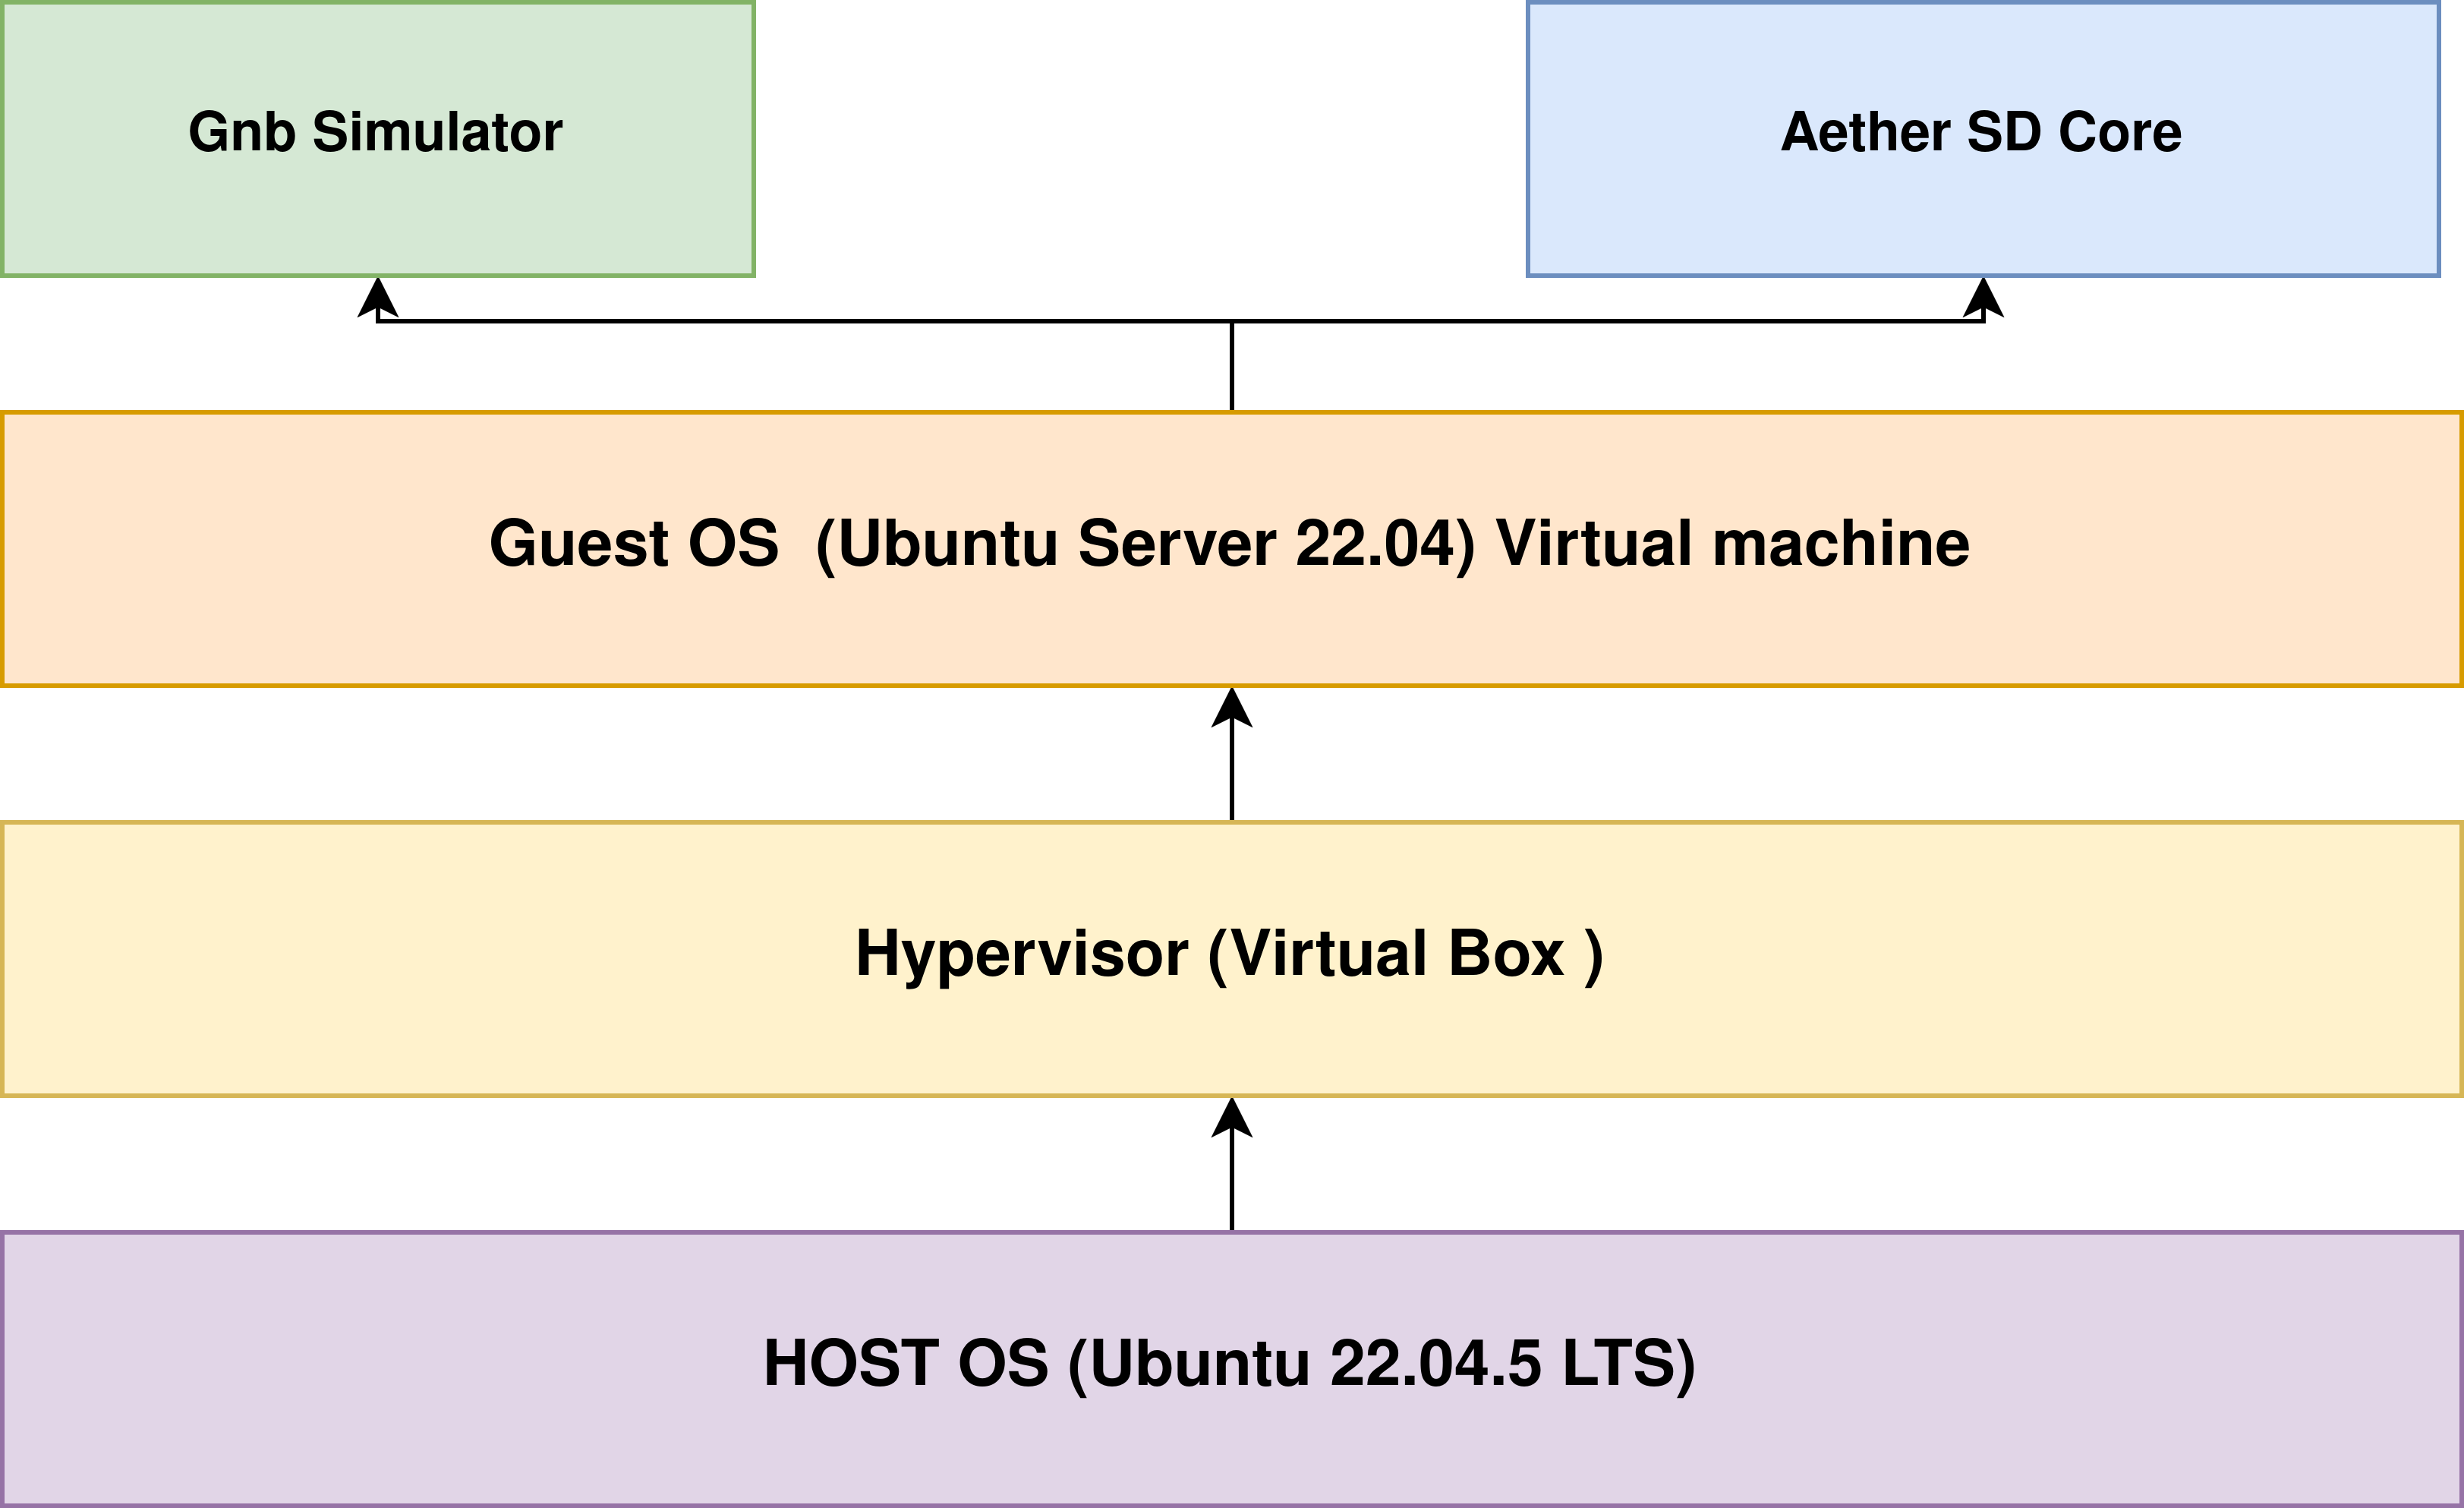
\includegraphics[keepaspectratio=true, width=\textwidth]{Hassan_Thesis/images/Single Vm/Deployment&Netwroking/Quick Start Deployment-Deployment Overview.png}
    \caption{Deployment Overview for Quick Start Setup.}
    \label{fig:quick-start-deployment-overview}
\end{figure}

As depicted in Figure \ref{fig:quick-start-deployment-overview}, the deployment consists of four main layers:

\begin{itemize}
    \item \textbf{Host OS:} The host operating system is Ubuntu 22.04.5 LTS, which serves as the base layer for running the hypervisor.
    \item \textbf{Hypervisor:} Oracle VirtualBox acts as the hypervisor, providing the necessary abstraction to run the guest operating system.
    \item \textbf{Guest OS:} The guest operating system is Ubuntu Server 22.04, running within the virtual machine. This layer hosts the Aether SD-Core and gNBsim components.
    \item \textbf{Components:} Within the guest OS, two key components are deployed:
    \begin{itemize}
        \item \textbf{Aether SD-Core:} The Software-Defined Core Network responsible for managing 5G core functionalities.
        \item \textbf{gNBsim:} A 5G simulator used to mimic real-world network interactions and evaluate 5G functionalities.
    \end{itemize}
\end{itemize}

This layered approach allows for a controlled and isolated environment to deploy and test Aether SD-Core and gNBsim. By utilizing a single VM on a personal laptop, the setup enables researchers to observe performance bottlenecks and assess the feasibility of deploying private 5G solutions in a constrained system.

\subsubsection{Purpose of the Quick Start Deployment}

The Quick Start deployment focuses on evaluating the fundamental aspects of Aether SD-Core in a minimalistic setup. Key objectives include:

\begin{itemize}
    \item Testing \textbf{UE registration} and \textbf{PDU session establishment} using gNBsim.
    \item Measuring \textbf{latency} and \textbf{response times} for critical call flows.
    \item Identifying \textbf{performance bottlenecks} caused by resource constraints in the virtualized environment.
\end{itemize}

This setup serves as a baseline for more advanced deployments, providing insights into the scalability and reliability of Aether in resource-constrained scenarios.


\subsection{Full Aether Deployment (Lab PC)}

The full-scale Aether deployment was conducted on a high-performance Lab PC, enabling more advanced testing scenarios. This section describes the hardware specifications, virtual machine configurations, and overall deployment architecture for the Lab PC setup.

\subsubsection{Hardware Specifications}

Table \ref{tab:lab-pc-specs} details the specifications of the Lab PC used for the full-scale Aether deployment. The system features an Intel Core i7-12700 processor, 64 GB of RAM, and a 500 GB SSD. Oracle VirtualBox is used as the hypervisor to run multiple virtual machines, supporting both the core Aether platform and UERANSIM.

\begin{table}[htbp]
    \centering
    \caption{Lab PC Specifications}
    \label{tab:lab-pc-specs}
    \resizebox{0.9\textwidth}{!}{
    \begin{tabular}{p{4cm} p{10cm}}
        \toprule
        \textbf{Component} & \textbf{Specification} \\
        \midrule
        CPU & Intel Core i7-12700 (12 cores, 20 threads, up to 4.9 GHz) \\
        RAM & 64 GB \\
        Storage & 500 GB SSD (457 GB partition, 408 GB used, 28 GB free) \\
        Operating System & Ubuntu 22.04.5 LTS \\
        Kernel & Linux 6.8.0-52-generic \\
        Hypervisor & Oracle VirtualBox \\
        \bottomrule
    \end{tabular}
    }
\end{table}

\subsubsection{Virtual Machine Configuration}

Two virtual machines were deployed to facilitate the full Aether platform and UERANSIM components. The first VM hosts the Aether platform core services, while the second VM runs UERANSIM for simulating 5G gNB and UE functionalities.

\begin{table}[htbp]
    \centering
    \caption{Aether Platform Core Deployment VM Specifications}
    \label{tab:aether-vm}
    \resizebox{0.9\textwidth}{!}{
    \begin{tabular}{p{4cm} p{10cm}}
        \toprule
        \textbf{VM Parameter} & \textbf{Specification} \\
        \midrule
        Purpose & Core deployment of Aether platform components \\
        OS & Ubuntu Server 22.04 \\
        CPU & 20 vCPUs \\
        RAM & 40 GB \\
        Storage & Virtual Disk (VMDK, dynamically allocated) \\
        Network Adapter & Host-only Adapter (vboxnet0) \\
        \bottomrule
    \end{tabular}
    }
\end{table}

\begin{table}[htbp]
    \centering
    \caption{UERANSIM VM Configuration}
    \label{tab:ueransim-vm}
    \resizebox{0.9\textwidth}{!}{
    \begin{tabular}{p{4cm} p{10cm}}
        \toprule
        \textbf{VM Parameter} & \textbf{Specification} \\
        \midrule
        Purpose & Simulate 5G User Equipment and Radio Access Network \\
        OS & Ubuntu Server 22.04 \\
        CPU & 3 vCPUs \\
        RAM & 10 GB \\
        Storage & Virtual Disk (VMDK, dynamically allocated) \\
        Network Adapters & Adapter 1: NAT Network (internet connectivity) \\
                         & Adapter 2: Host-only Adapter (vboxnet0) \\
        \bottomrule
    \end{tabular}
    }
\end{table}

The Aether Platform Core Deployment VM provides the underlying Kubernetes environment for deploying multiple Aether blueprints, including the SD-Core, Runtime Operation Control (ROC), and associated monitoring components. The UERANSIM VM, on the other hand, is responsible for simulating 5G radio and user equipment functionalities, enabling realistic testing of the end-to-end 5G core network.

\subsubsection{Deployment Overview}

Figure~\ref{fig:lab-pc-deployment-overview} presents a high-level architecture of the Full Aether Deployment on the Lab PC. As in the Quick Start setup, the diagram illustrates the layering from the host operating system down to the virtualized components, but with two separate virtual machines to accommodate more advanced testing scenarios.

\begin{figure}[!htb]
    \centering
    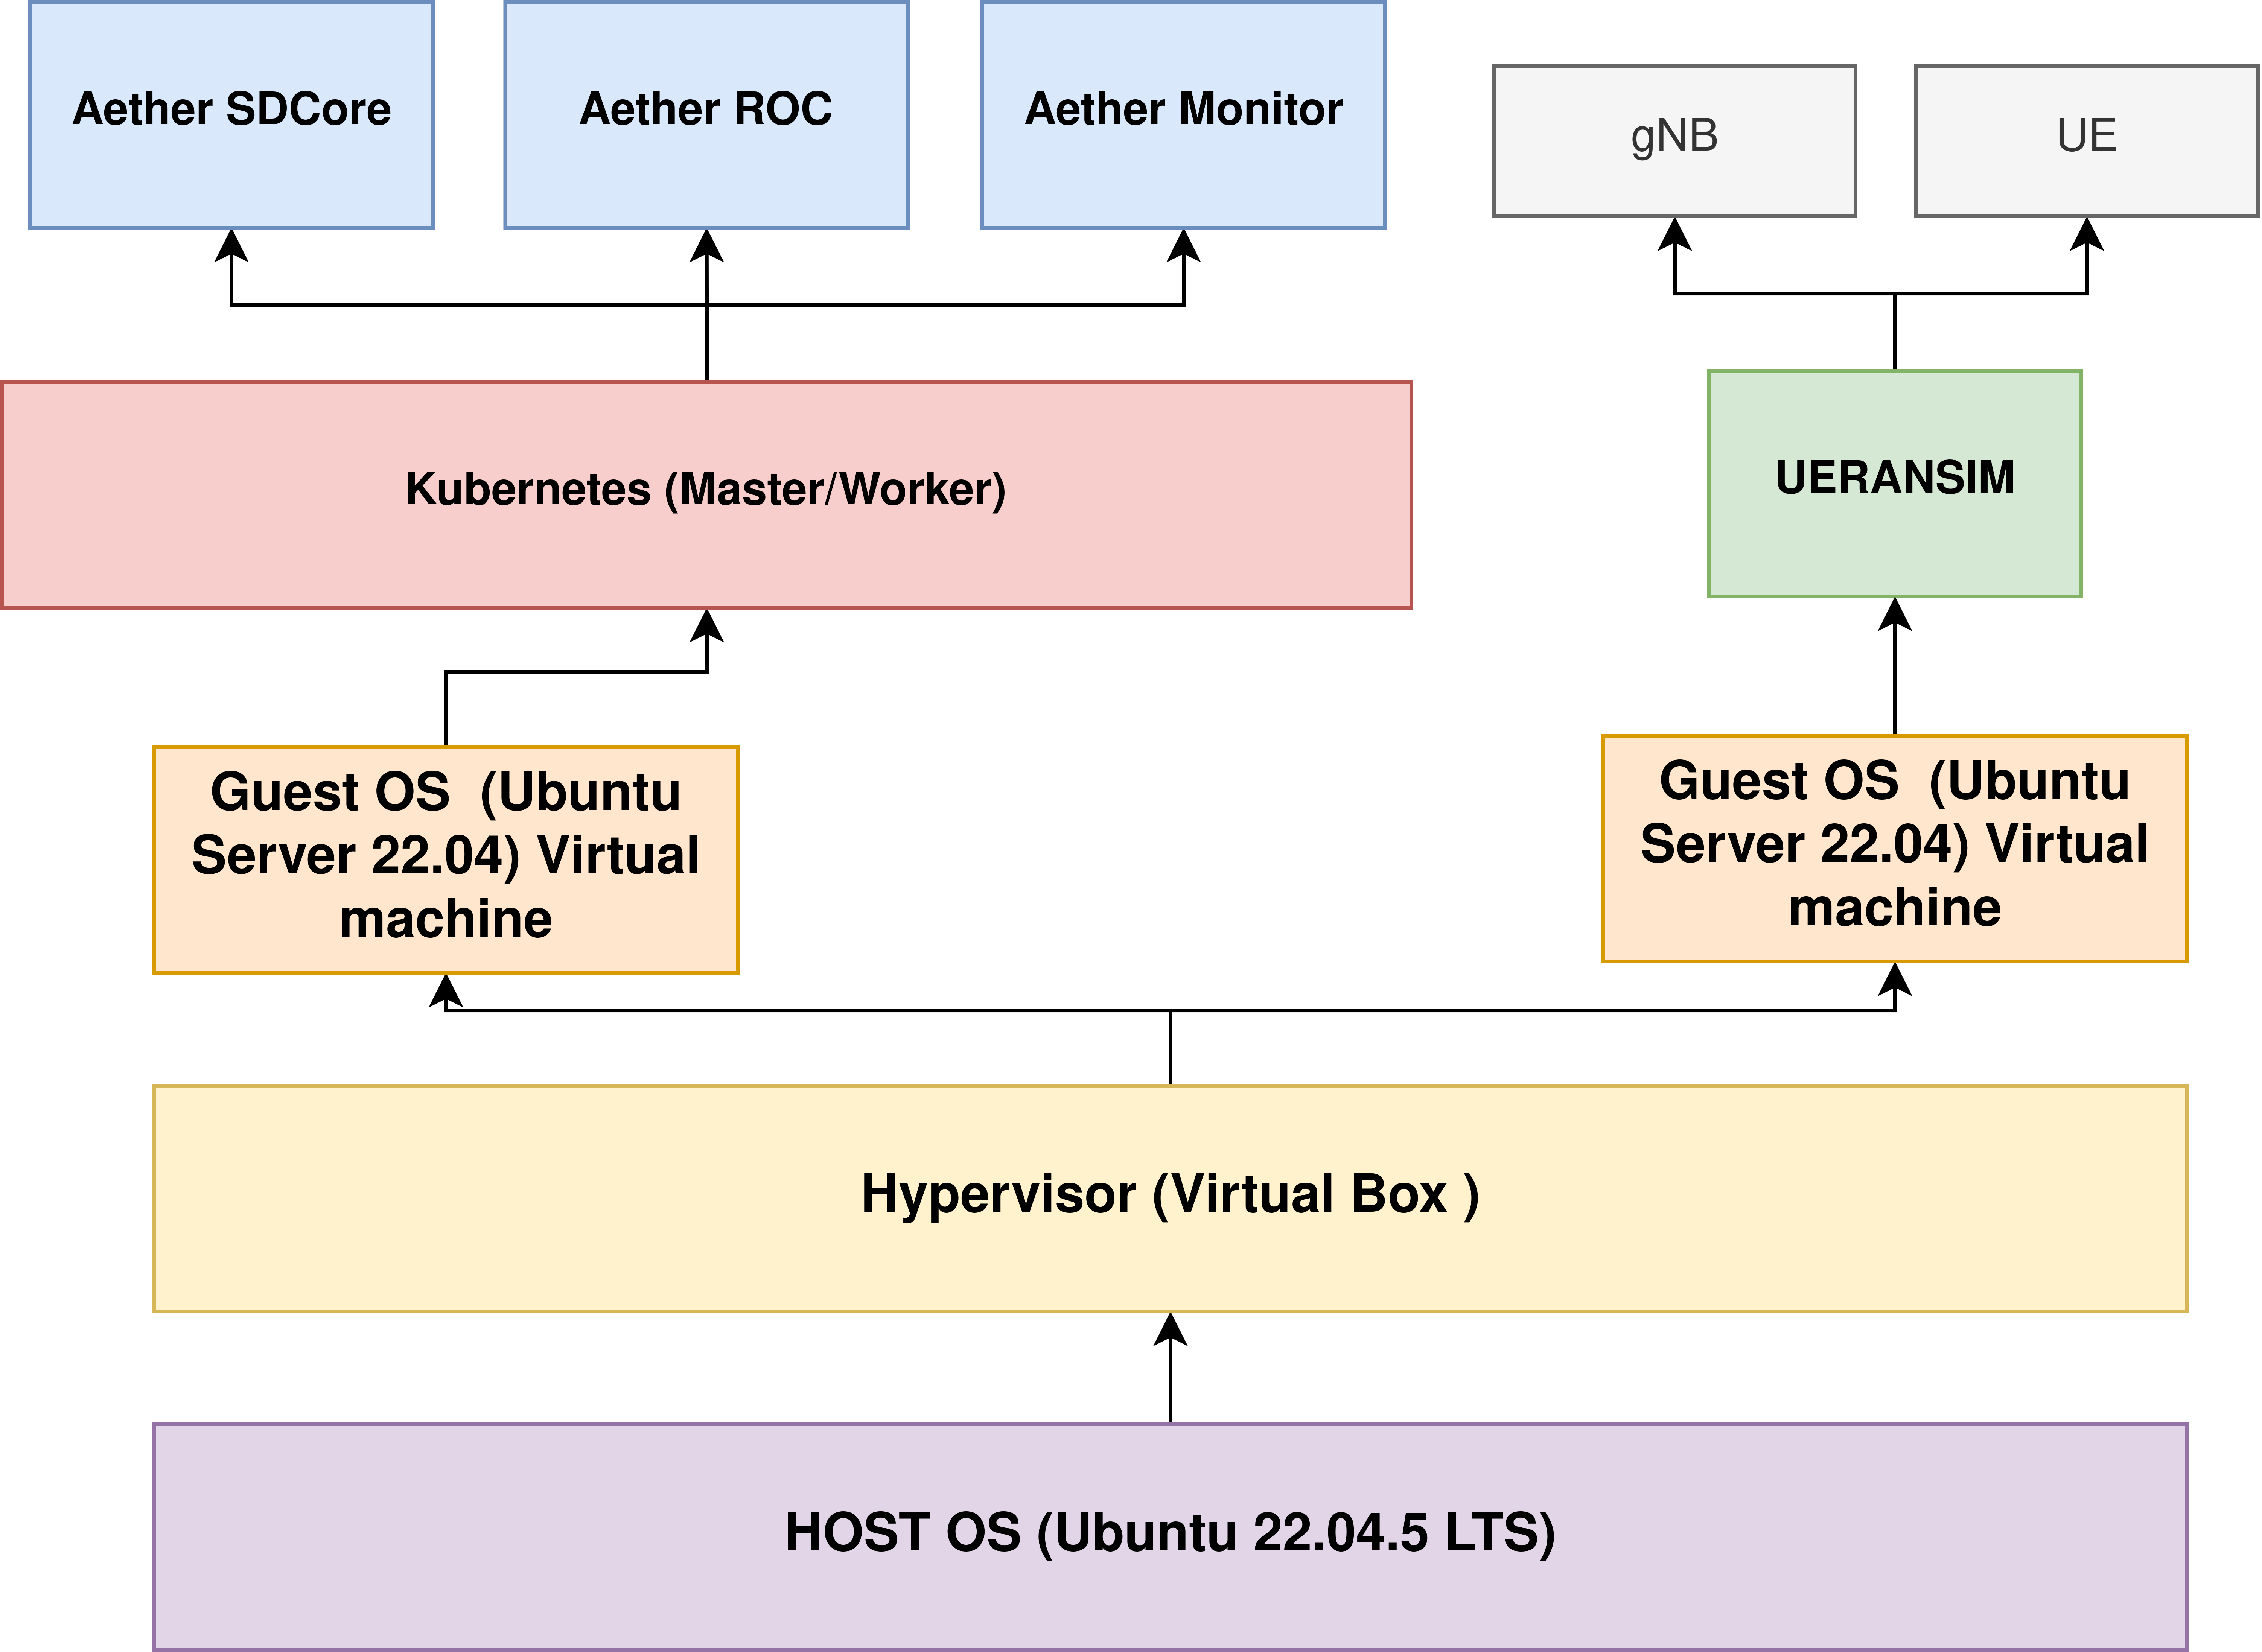
\includegraphics[keepaspectratio=true, width=\textwidth]{Hassan_Thesis/images/LAB PC/Deployment&Netwroking/Lab PC Deployment Overview.png}
    \caption{Deployment Overview for Full Aether Setup.}
    \label{fig:lab-pc-deployment-overview}
\end{figure}

As depicted in Figure~\ref{fig:lab-pc-deployment-overview}, the deployment consists of the following layers:

\begin{itemize}
    \item \textbf{Host OS (Ubuntu 22.04.5 LTS):} 
    The base operating system running on the Lab PC, providing the platform for the hypervisor.
    \item \textbf{Hypervisor (Oracle VirtualBox):} 
    Responsible for abstracting hardware resources and managing the guest operating systems.
    \item \textbf{Guest OS (Two Separate VMs):} 
    \begin{itemize}
        \item \textbf{Aether Platform Core VM:} 
        Hosts the Aether SD-Core, Aether ROC, Aether Monitor, and other supporting microservices. 
        \item \textbf{UERANSIM VM:} 
        Simulates the 5G gNB and UE, enabling end-to-end testing of 5G call flows, QoS management, and runtime operations.
    \end{itemize}
    \item \textbf{Aether Components:} 
    \begin{itemize}
        \item \textbf{Aether SD-Core:} 
        Manages the 5G core functionalities, including AMF, SMF, UPF, and more.
        \item \textbf{Aether ROC:} 
        Provides Runtime Operation Control, enabling dynamic parameter modifications and policy enforcement.
        \item \textbf{Aether Monitor:} 
        Collects metrics and performance data for real-time and historical analysis.
        \item \textbf{UERANSIM (gNB + UE):} 
        Emulates the radio interface and user equipment, allowing for realistic testing of registration, PDU sessions, and QoS flows.
    \end{itemize}
\end{itemize}

This multi-VM architecture allows for a clearer separation of core network services and simulated radio components, facilitating more complex scenarios and improved resource management compared to the single VM setup.

\subsubsection{Purpose of the Full Aether Deployment}

The Full Aether Deployment on the Lab PC aims to explore advanced features and stress-test the Aether platform in a more resource-rich environment. Key objectives include:

\begin{itemize}
    \item \textbf{Multiple Blueprint Deployment:}  
    Evaluating the SD-Core alongside other Aether services, such as Runtime Operation Control and additional UPFs.

    \item \textbf{QoS Testing:}  
    Investigating how multiple UPFs and QoS policies impact latency, throughput, and overall network performance.

    \item \textbf{Dynamic Parameter Modification:}  
    Observing how Runtime Operation Control can adjust parameters (e.g., slice configuration, policy rules) during runtime.
\end{itemize}


By leveraging a high-performance Lab PC and multiple VMs, this deployment provides a robust environment for validating the scalability, resilience, and feature set of the Aether platform. The insights gained from this setup help inform real-world private 5G deployments and further research into 5G network slicing and orchestration.




\section{Deployment Process}
\label{sec:deployment-process}

The deployment process for the Aether platform was conducted in two distinct phases: 
\begin{enumerate}
    \item \textbf{Quick Start Deployment (Personal Laptop)}: A minimal yet functional setup designed to demonstrate basic 5G core functionalities using a single virtual machine (VM).
    \item \textbf{Full Aether Deployment (Lab PC)}: A more comprehensive and feature-rich environment leveraging multiple VMs to support advanced testing scenarios, including runtime operation control (ROC), Quality of Service (QoS) management, and dedicated monitoring services.
\end{enumerate}

Each phase builds upon the previous one, starting with a simplified setup on a personal laptop and progressing to a robust multi-VM architecture on a Lab PC. The following sections provide a detailed breakdown of both deployments, their network topologies, and key interactions.

---

\subsection{Quick Start Deployment (Personal Laptop)}
\label{subsec:quickstart-deployment}

\subsubsection{Overview}
\label{subsubsec:qs-overview}

The Quick Start Deployment serves as an introductory setup, demonstrating the fundamental functionalities of a 5G core network. This deployment utilizes a single VM hosted on a personal laptop, integrating the \textbf{SD-Core} (including AMF, SMF, UDM, and UPF) alongside \textbf{gNBsim}. By consolidating all components into a single environment, this setup provides a straightforward platform for initial testing and demonstration of 5G call flows, user registration, and basic data-plane interactions.

\newpage
\subsubsection{Networking Diagram}
\label{subsubsec:qs-networking-diagram}
Figure~\ref{fig:quick-start-networking-diagram} illustrates the networking topology for the Quick Start deployment. The diagram highlights the role of the \texttt{DATA\_IF} interface, which connects to the internet, and the \texttt{gnbaccess} bridge, which facilitates communication between the \texttt{gNBsim} container and the core network.

\begin{figure}[H]
    \centering
    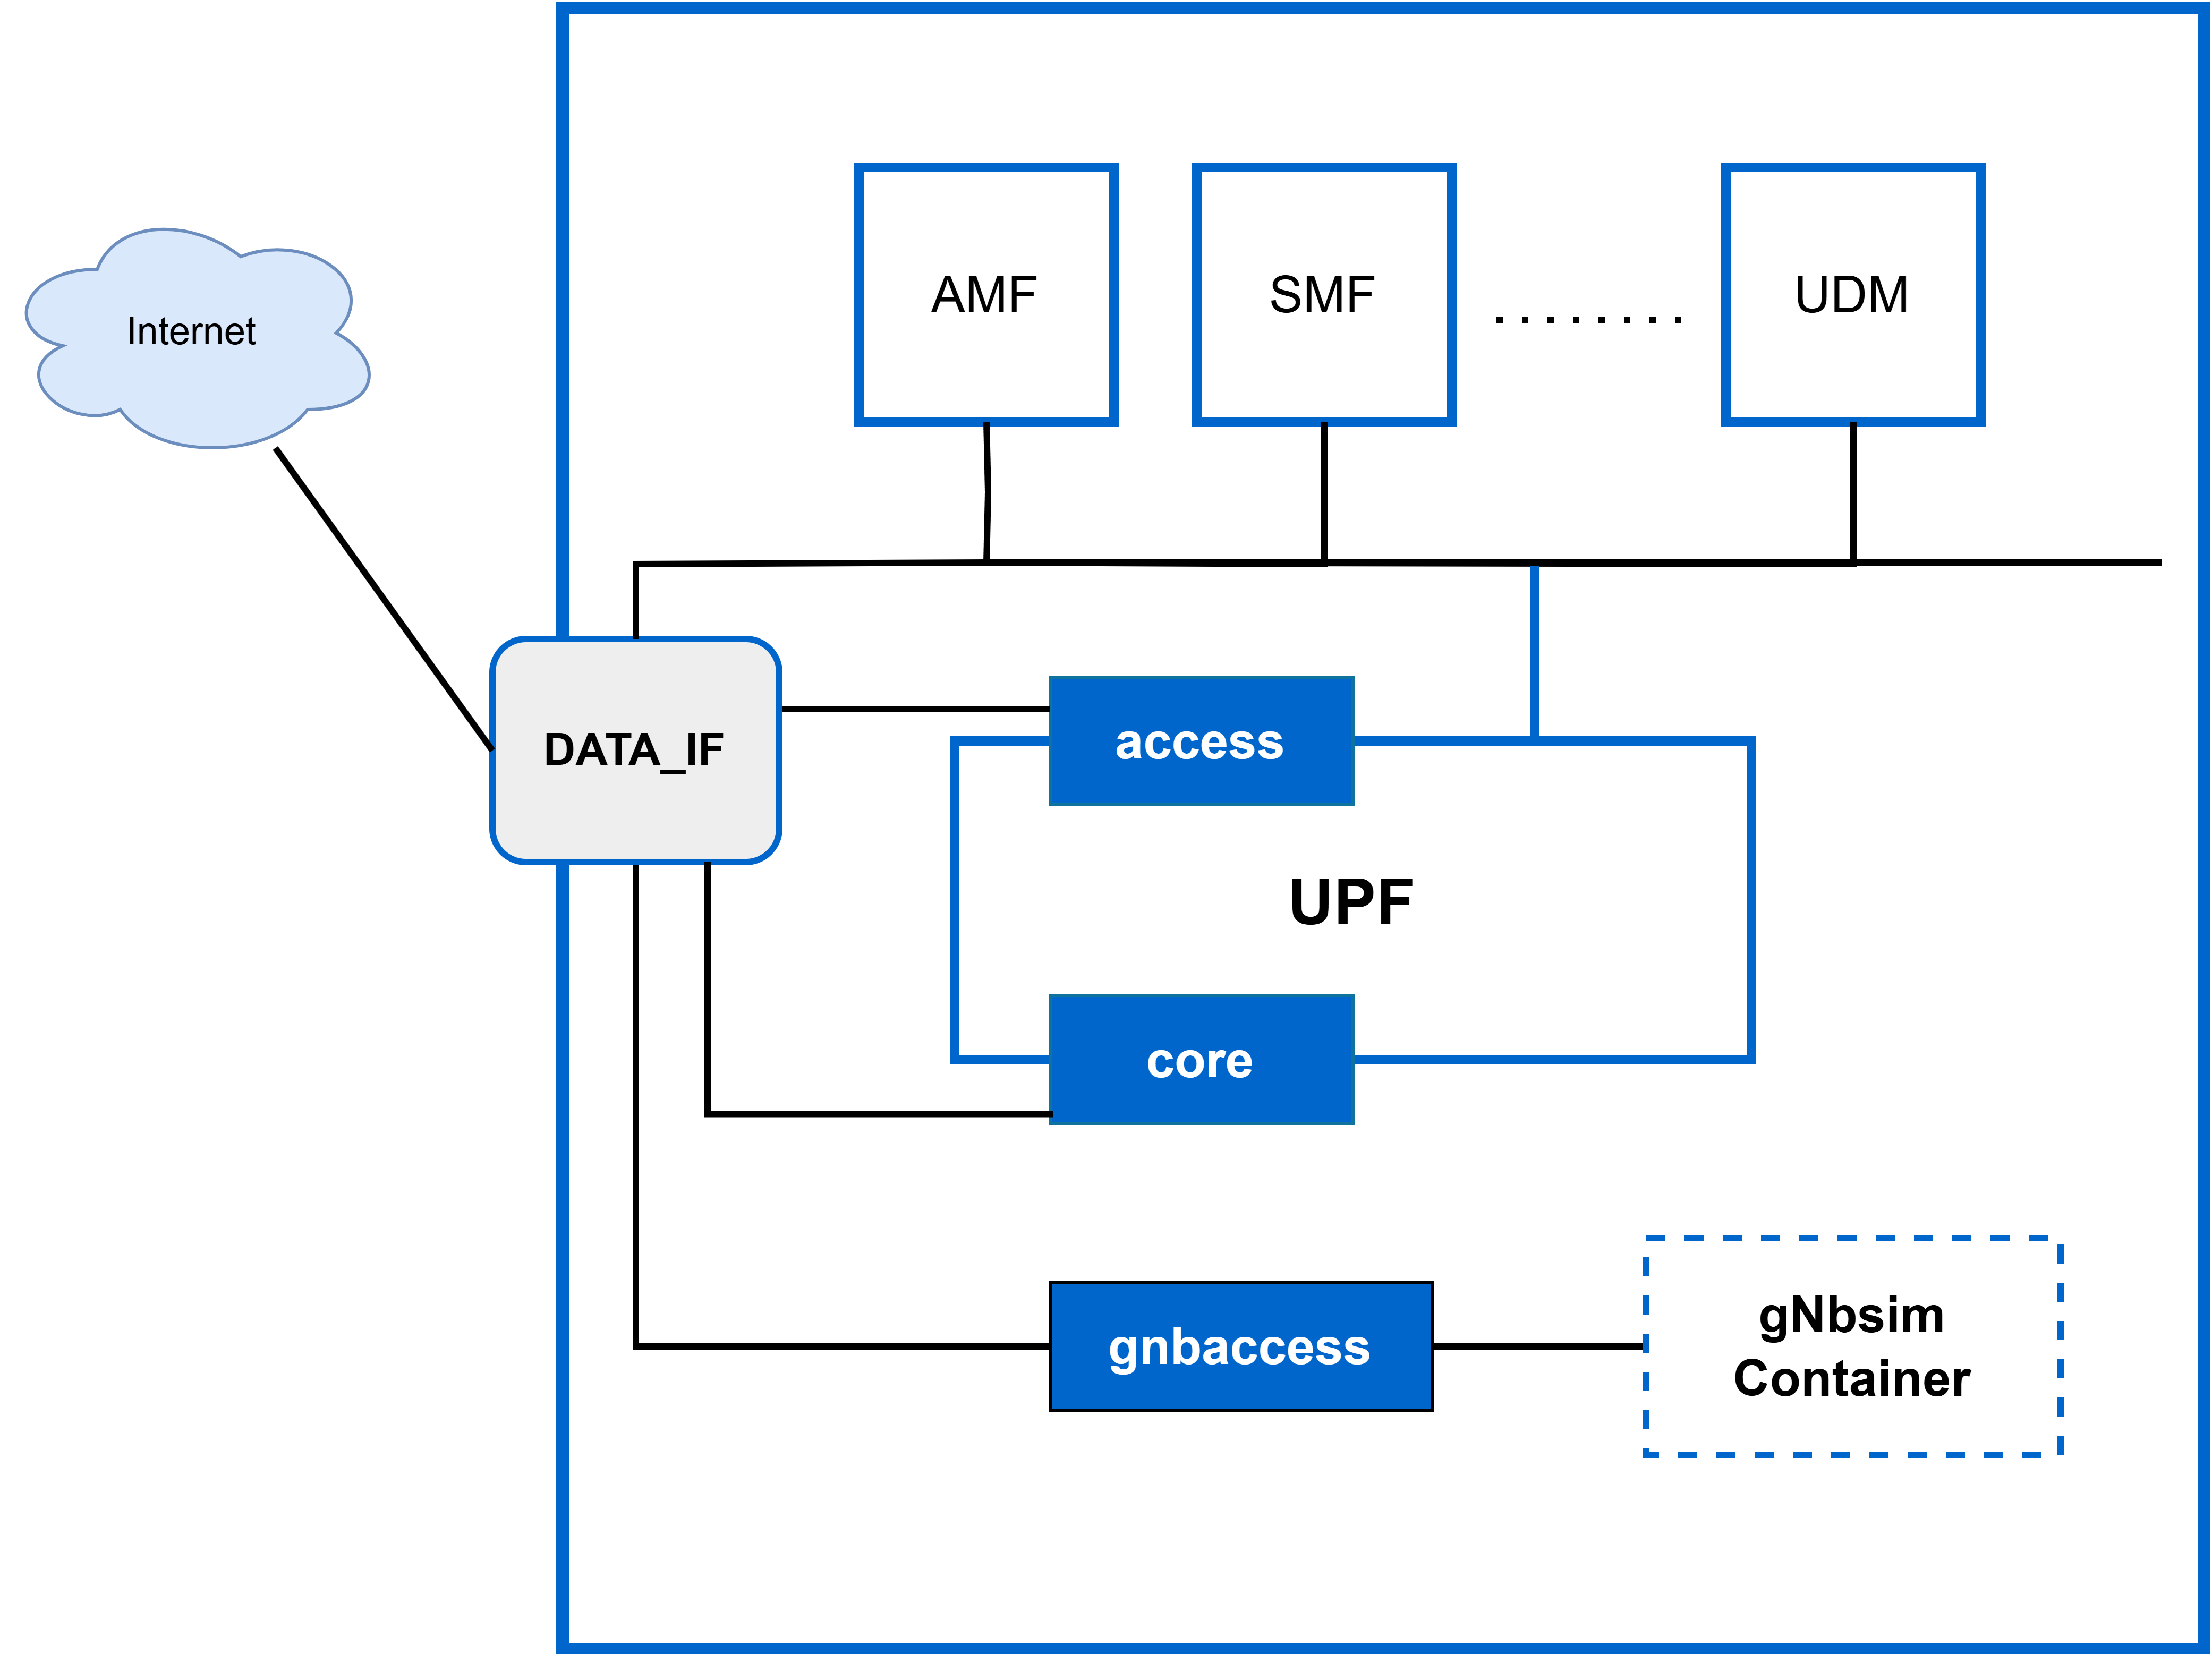
\includegraphics[keepaspectratio=true, width=0.9\textwidth]{Hassan_Thesis/images/Single Vm/Deployment&Netwroking/Quick Start Deployment-Netwroking Diagram.png}
    \caption{Networking Diagram for Quick Start Deployment.}
    \label{fig:quick-start-networking-diagram}
\end{figure}

\begin{table}[H]
\centering
\caption*{Key Table for Figure~\ref{fig:quick-start-networking-diagram} – Networking Diagram for Quick Start Deployment}
\renewcommand{\arraystretch}{1.3}
\begin{tabular}{@{}p{4cm}>{\raggedright\arraybackslash}p{10cm}@{}}
\toprule
\textbf{Symbol / Color} & \textbf{Meaning} \\
\midrule
{\textbf{Blue Boxes}} & Virtual network bridges/interfaces (\texttt{access}, \texttt{core}, \texttt{gnbaccess}) implemented using Linux bridges and Macvlan. \\
\textbf{White Boxes} & Core 5G components (e.g., \texttt{AMF}, \texttt{SMF}, \texttt{UDM}) deployed as Docker containers orchestrated by Kubernetes. \\
{\textbf{Dashed blue Box}} & \texttt{gNBsim} container, a standalone Docker container outside Kubernetes orchestration. \\
\textbf{Bold Black Lines} & Logical data path connections between network components. \\
\texttt{DATA\_IF} Box & External interface for data traffic to and from the internet. \\
\bottomrule
\end{tabular}
\end{table}

As shown in Figure~\ref{fig:quick-start-networking-diagram}, the key components of this deployment include:
\begin{itemize}
    \item \textbf{Internet Connection}: The \texttt{DATA\_IF} interface provides external connectivity.
    \item \textbf{UPF (User Plane Function)}:Acts as the entry point for user data traffic within the 5G core. It is responsible for forwarding, routing, and packet inspection of user-plane data between the RAN and external networks. In this deployment, the UPF bridges data packets between the core network and the internet by connecting the N3 interface (from the gNB) to the N6 interface (towards the internet). It also supports functionalities such as Quality of Service (QoS) enforcement.
    \item \textbf{Core Network Components (AMF, SMF, UDM etc.)}:The 5G Core Control Plane consists of modular software components called Network Functions (NFs), each responsible for a specific control task. In this deployment, these NFs—such as AMF, SMF, UDM, NRF, AUSF, PCF, NSSF, and NAF—are each deployed as lightweight Docker containers, orchestrated by Kubernetes for scalability and manageability. These components communicate over standardized interfaces (e.g., N1, N11, N8, N10, N12) to perform control-plane tasks such as:

AMF (Access and Mobility Management Function): Handles user equipment (UE) registration, mobility management, and session access authorization.
SMF (Session Management Function): Manages PDU sessions, IP address allocation, and interfaces with the UPF.
UDM (Unified Data Management): Stores subscriber data and exposes it to other functions like AMF and AUSF.
AUSF (Authentication Server Function): Authenticates UEs in coordination with the UDM.
NRF (Network Repository Function): Acts as a service registry, allowing NFs to discover and communicate with each other dynamically.
PCF (Policy Control Function): Provides policy rules related to QoS, charging, and access control.
NSSF (Network Slice Selection Function): Assists in selecting the appropriate network slice for a given session.
NAF (NEF Application Function): Interfaces with application functions and exposes 5G capabilities via APIs.

This microservices-based architecture enables high flexibility and cloud-native scalability, aligning with the 5G core's service-based architecture (SBA) principles.

\item \textbf{gNBsim Container}: A standalone Docker container (outside Kubernetes) that emulates a 5G gNodeB (gNB). It interacts with the 5G Core over the N2 (control plane) and N3 (user plane) interfaces, enabling end-to-end testing of key 5G procedures such as UE registration, PDU session establishment, and Quality of Service (QoS) enforcement. The gNBsim generates control and user plane traffic, allowing validation of core network behavior under simulated radio access conditions without requiring real hardware.

\end{itemize}





\subsubsection{Detailed Networking Diagram}
\label{subsubsec:qs-detailed-network}

Figure~\ref{fig:quick-start-networking} provides a more granular view of the Quick Start deployment, illustrating how traffic flows among the physical interface (\texttt{enp0s3}), the \texttt{access} and \texttt{core} bridges, and the \texttt{UPF} container.

\begin{figure}[H]
    \centering
    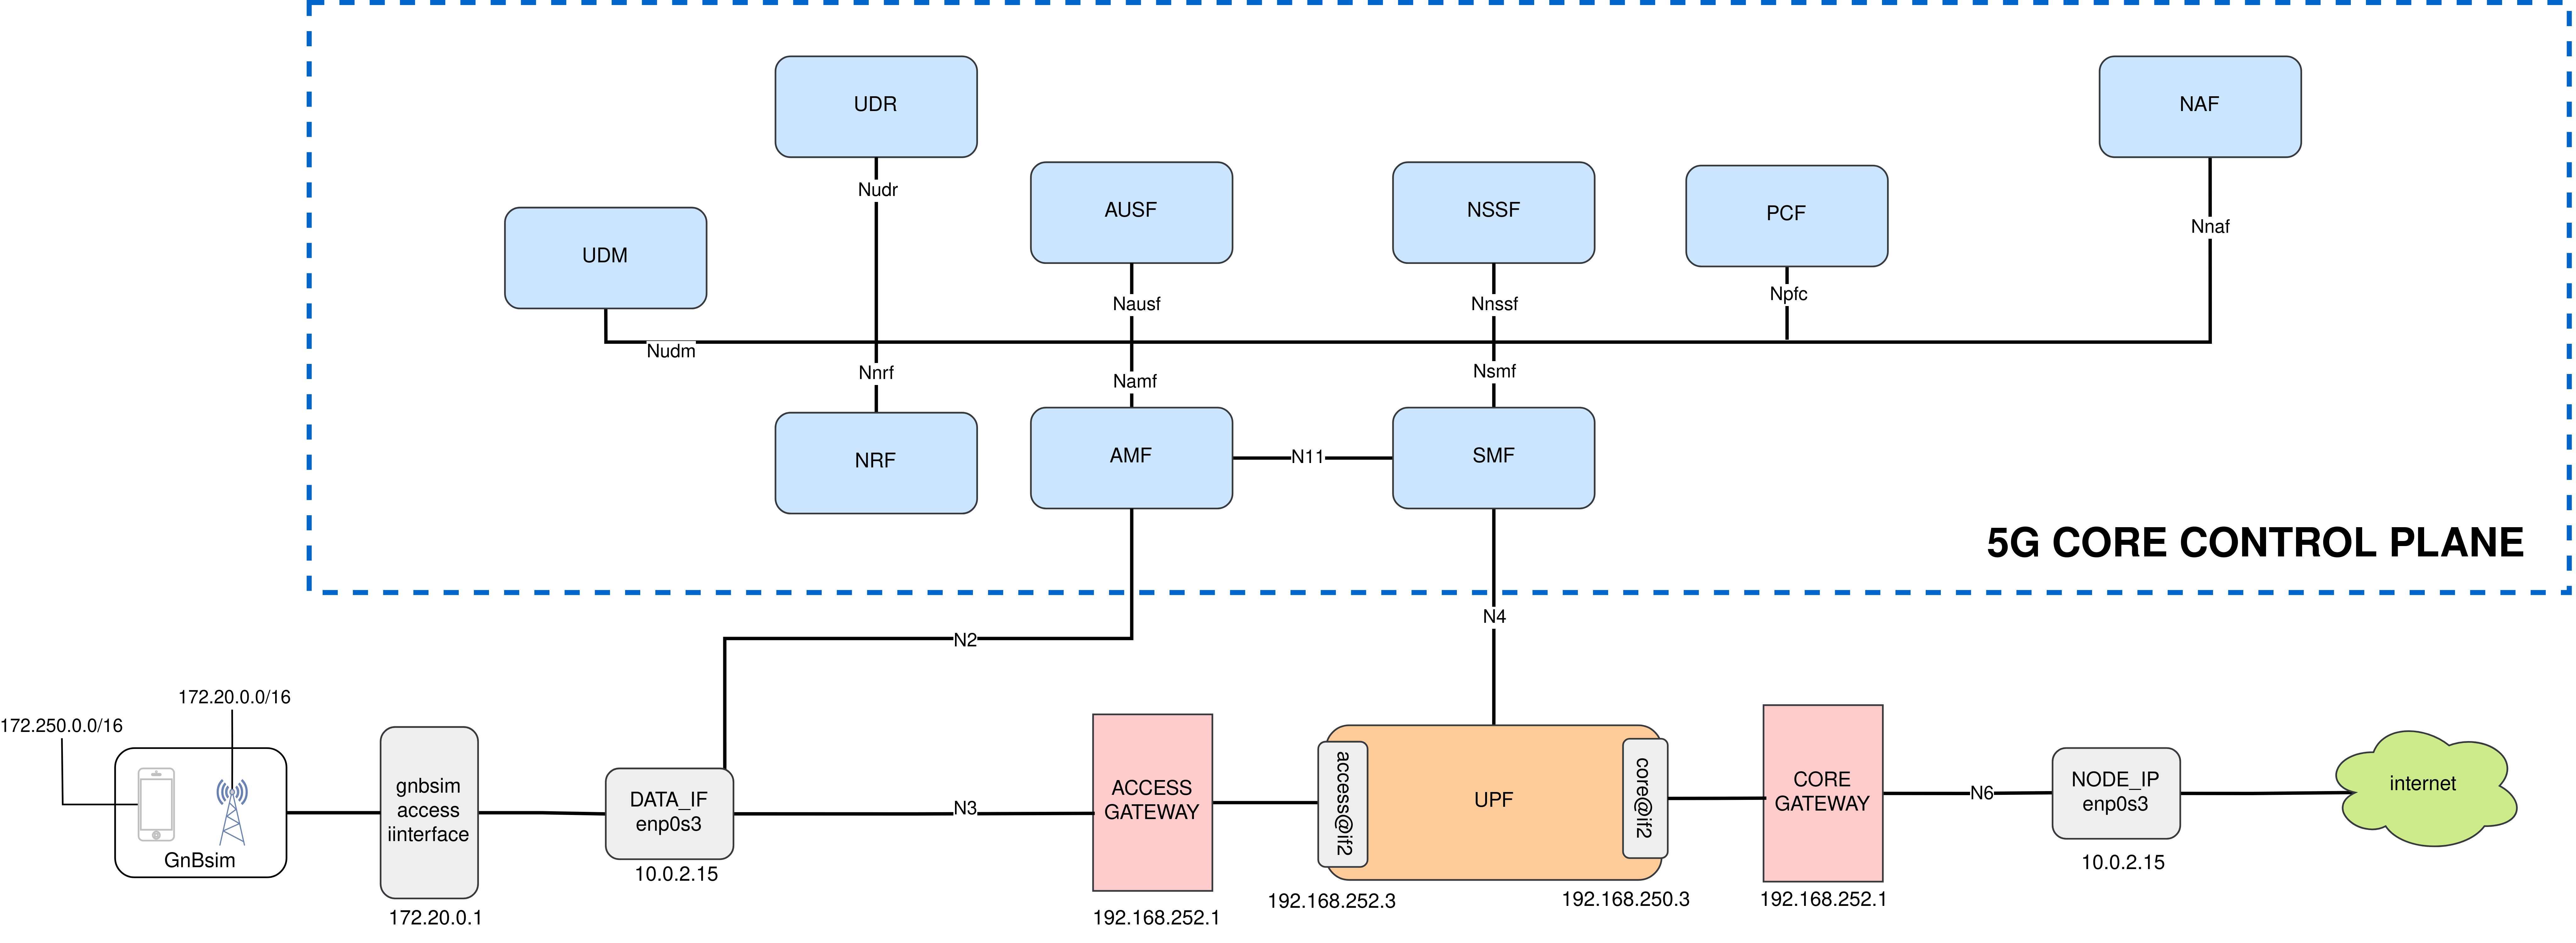
\includegraphics[keepaspectratio=true, width=0.9\textwidth]{Hassan_Thesis/images/Single Vm/Deployment&Netwroking/Quick Start Deployment-Detailed Networking Diagram.png}
    \caption{Detailed Networking Diagram for Quick Start Deployment.}
    \label{fig:quick-start-networking}
\end{figure}

\textbf{Key Elements:}
\begin{itemize}
    \item \textbf{gNBsim Container}: A standalone Docker container that emulates a gNodeB (gNB). It generates GTP-encapsulated traffic and communicates with the UPF over the N3 interface via the \texttt{access} bridge.
    
    \item \textbf{gnbsim Access Interface}: A Macvlan-based virtual interface that connects the gNBsim container to the UPF's \texttt{access} bridge, enabling N3 interface traffic exchange.

    \item \textbf{Access Bridge}: A Linux bridge that connects the UPF downstream to the Radio Access Network (RAN), representing the 3GPP-defined N3 interface.

    \item \textbf{UPF (User Plane Function)}: A key data plane component that removes or adds GTP headers and routes user traffic between the RAN (via N3) and the internet (via N6).

    \item \textbf{Core Bridge}: A Linux bridge that connects the UPF upstream to the external network, corresponding to the N6 interface defined in 3GPP.

    \item \textbf{Physical Interface (\texttt{enp0s3})}: The host machine’s external network interface, used by the UPF and Core Gateway to reach the internet.

    \item \textbf{Internet}: The destination or source of user traffic, representing external services accessible via the 5G Core.
\end{itemize}


\subsubsection{Key Interactions}
\label{subsubsec:qs-key-interactions}

The Quick Start Deployment involves two primary types of interactions:

\begin{itemize}
    \item \textbf{Data Flow}: User data flows from the internet through the \texttt{DATA\_IF} interface to the UPF. The UPF then routes the packets to the \texttt{gNBsim} container via the \texttt{access} bridge.
    \item \textbf{Signaling Flow}: Signaling messages are exchanged between the \texttt{gNBsim} container and the core network components (AMF, SMF, UDM) via the \texttt{gnbaccess} bridge. These interactions support tasks such as user registration, session establishment, and IP address allocation.
\end{itemize}

\subsubsection{Packet Flow Analysis}
\label{subsubsec:qs-packet-flow}

\paragraph{Upstream Flow (gNB $\rightarrow$ Internet)}
\begin{itemize}
    \item The \texttt{gNBsim} container sends GTP-encapsulated packets to the UPF’s \texttt{access} interface (\texttt{192.168.252.3}).
    \item The UPF removes the GTP headers and forwards the raw IP packets to its \texttt{core} interface.
    \item Packets exit to the internet via the physical interface (\texttt{enp0s3}), with source NAT applied as needed to ensure private UE IPs remain hidden.
\end{itemize}

\paragraph{Downstream Flow (Internet $\rightarrow$ gNB)}
\begin{itemize}
    \item Incoming packets arrive on the physical interface (\texttt{enp0s3}) from the internet.
    \item The UPF encapsulates these packets with GTP headers and sends them to the \texttt{gNBsim} container over the \texttt{access} bridge.
\end{itemize}

\subsubsection{Benefits of the Setup}
\label{subsubsec:qs-benefits}

The Quick Start Deployment offers several advantages:
\begin{itemize}
    \item \textbf{Realistic Simulation}: The use of \texttt{access} and \texttt{core} bridges ensures realistic simulation of 5G network interactions, enabling comprehensive testing of UPF functionality.
    \item \textbf{Simplified Configuration}: All components (SD-Core, gNBsim, UPF) reside in a single VM, streamlining deployment and reducing complexity.
    \item \textbf{Resource Efficiency}: The single-VM setup is optimized for constrained environments like personal laptops, making it accessible for initial experimentation.
\end{itemize}

---

\subsection{Full Aether Deployment (Lab PC)}
\label{subsec:full-aether-deployment}

\subsubsection{Overview}
\label{subsubsec:labpc-overview}

Building on the foundation of the Quick Start Deployment, the Full Aether Deployment introduces a more sophisticated and scalable environment on a Lab PC. This deployment leverages multiple virtual machines (VMs) to host the SD-Core, Aether Runtime Operation Control (ROC), multiple User Plane Functions (UPFs), and dedicated monitoring services. This multi-VM architecture supports advanced runtime control, QoS management, and in-depth performance analysis, enabling the exploration of complex 5G scenarios.

\subsubsection{Networking Diagram}
\label{subsubsec:labpc-network-diagram}

Figure~\ref{fig:lab-pc-network} illustrates the networking setup for the Full Aether Deployment. The diagram highlights the interaction between the UERANSIM container (simulating user equipment and gNodeB behavior), multiple UPFs (UPF0, UPF1), the core network (AMF, SMF, UDM), and the external internet.

\begin{figure}[!htb]
    \centering
    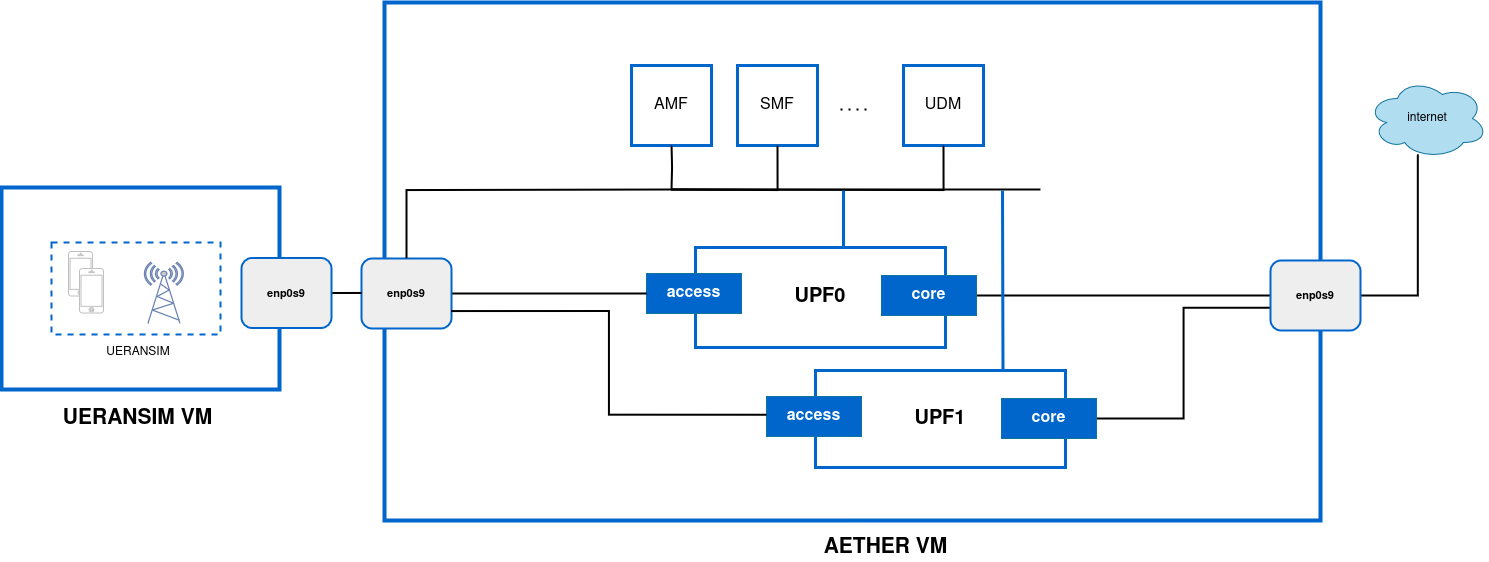
\includegraphics[keepaspectratio=true, width=0.9\textwidth]{Hassan_Thesis/images/LAB PC/Deployment&Netwroking/LAB PC Netwroking Diagram.png}
    \caption{Networking Diagram for Full Aether Deployment on the Lab PC.}
    \label{fig:lab-pc-network}
\end{figure}

As depicted in Figure~\ref{fig:lab-pc-network}, the key components of this deployment include:
\begin{itemize}
    \item \textbf{UERANSIM (UE Simulation)}: Emulates gNB + UE behavior via the \texttt{enp0s9} interface, enabling realistic testing of registration, session establishment, and data exchange.
    \item \textbf{Core Network (AMF, SMF, UDM)}: Manages authentication, session establishment, and subscriber data.
    \item \textbf{Multiple UPFs (UPF0, UPF1)}: Each UPF handles user-plane traffic through \texttt{access} and \texttt{core} interfaces, supporting multi-path scenarios and load balancing.
    \item \textbf{Internet Connection}: The core network connects to the external internet via the Lab PC’s physical interface (\texttt{enp0s9}), enabling end-to-end traffic flows.
\end{itemize}

\subsubsection{Detailed Components and Interactions}
\label{subsubsec:labpc-components}

\paragraph{Virtual Machines (VMs)}
\begin{itemize}
    \item \textbf{VM1}: Hosts the SD-Core (AMF, SMF, UDM), Aether ROC for runtime control, multiple UPFs for user-plane traffic management, and monitoring services for capturing performance metrics and enabling real-time troubleshooting.
    \item \textbf{VM2}: Dedicated to RAN simulation, running UERANSIM to emulate user equipment and gNodeB behavior.
\end{itemize}

\paragraph{Traffic Flow and Control Plane Interactions}
\begin{itemize}
    \item \textbf{UE Traffic Entry}: UERANSIM’s \texttt{enp0s9} interface provides the entry point for simulated UE data.
    \item \textbf{Core Network Processing}: The AMF, SMF, and UDM authenticate users, manage sessions, and store subscriber data.
    \item \textbf{Multi-UPF Handling}: The SMF selects either UPF0 or UPF1 for data routing, allowing testing of multi-path scenarios or load balancing.
    \item \textbf{Internet Egress}: Traffic exits to the internet via the Lab PC’s physical interface, with each UPF’s \texttt{core} interface handling GTP de-encapsulation.
\end{itemize}

\subsubsection{Detailed Networking Diagram}
\label{subsubsec:labpc-detailed-network}

Figure~\ref{fig:lab-pc-detailed-networking} provides a more granular view of the Full Aether Deployment, highlighting the interactions among various Aether platform services, runtime monitoring tools, and the multiple UPFs.

\begin{figure}[H] % 'p' forces placement on a dedicated page for floats
    \centering
    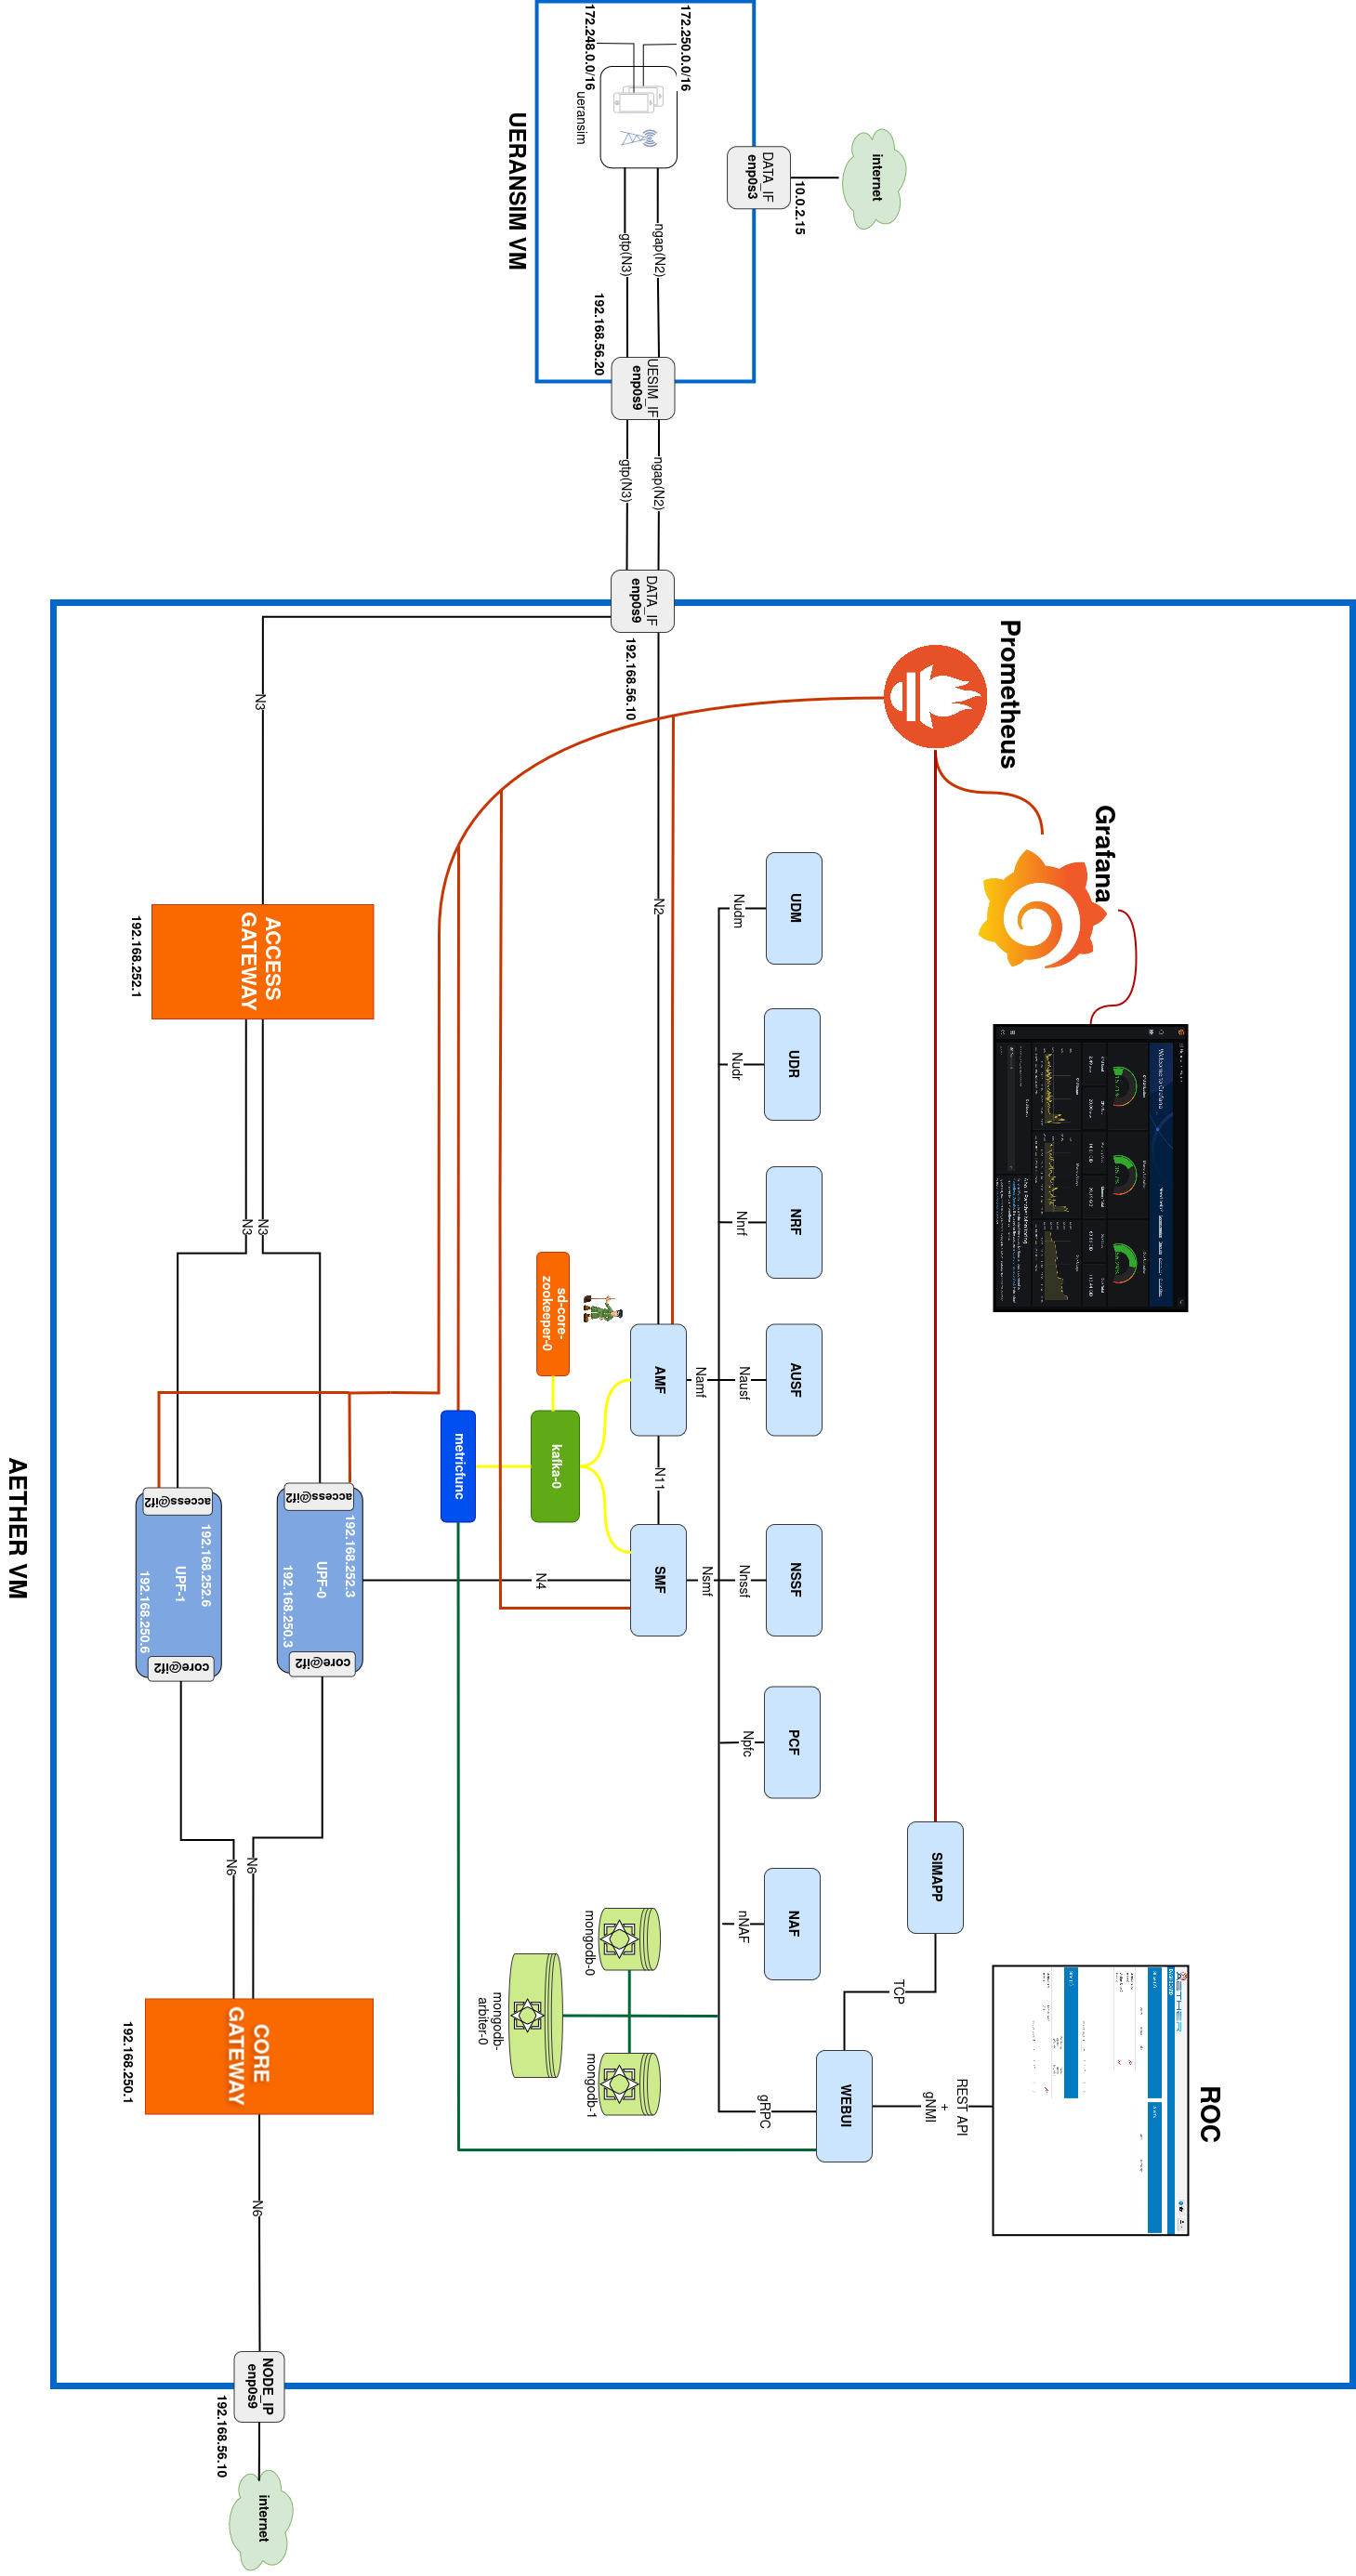
\includegraphics[width=\textwidth, height=\textheight, keepaspectratio]{Hassan_Thesis/images/LAB PC/Deployment&Netwroking/Lab PC Detailed Networking Diagram.png}
    \caption{Detailed Networking Diagram for Full Aether Deployment on the Lab PC.}
    \label{fig:lab-pc-detailed-networking}
\end{figure}


\textbf{Key Components and Interactions:}
\begin{itemize}
    \item \textbf{UERANSIM VM (Left Side)}:
    \begin{itemize}
        \item Simulates 5G User Equipment (UE) and gNodeB (gNB), generating both control-plane and user-plane traffic.
        \item Connects to the Aether VM via the \texttt{enp0s9} interface, enabling registration, session establishment, and data exchange.
    \end{itemize}
    \item \textbf{Aether VM (Center)}:
    \begin{itemize}
        \item Hosts the primary 5G core functions (AMF, SMF, UDM, PCF, NSSF) and multiple UPFs (\texttt{UPF0} and \texttt{UPF1}).
        \item Includes \textbf{Access Gateway} and \textbf{Core Gateway} components to route traffic from the RAN side (UERANSIM) to the internet, and vice versa.
        \item \textbf{Aether Runtime Operation Control (ROC)}: Dynamically manages slice configurations, QoS parameters, and network policies in real time.
    \end{itemize}
    \item \textbf{Monitoring and Visualization Tools (Top)}:
    \begin{itemize}
        \item \textbf{Prometheus}: Collects metrics from the core network components and UPFs.
        \item \textbf{Grafana}: Provides a graphical dashboard for real-time performance monitoring (e.g., throughput, latency, CPU/memory usage).
        \item \textbf{Syslog}: Captures events and logs from the Aether platform for troubleshooting and auditing.
    \end{itemize}
    \item \textbf{External Interfaces (Right Side)}:
    \begin{itemize}
        \item The \textbf{Core Gateway} connects the UPFs to the external internet, enabling data-plane traffic to flow from simulated UEs to external networks.
        \item The \texttt{enp0s9} interface represents a bridged or NATed connection to the Lab PC’s physical NIC, depending on the VirtualBox networking setup.
    \end{itemize}
\end{itemize}

\textbf{Traffic Flow Overview:}
\begin{itemize}
    \item \emph{UE-to-Internet (Upstream)}:
    \begin{itemize}
        \item UERANSIM (UE) transmits GTP-encapsulated packets through the Access Gateway to the selected UPF (\texttt{UPF0} or \texttt{UPF1}), where GTP headers are removed.
        \item The UPF forwards plain IP packets to the Core Gateway for egress to the internet.
    \end{itemize}
    \item \emph{Internet-to-UE (Downstream)}:
    \begin{itemize}
        \item Packets from the internet enter via the Core Gateway, reach the chosen UPF, and are then GTP-encapsulated before being sent to UERANSIM through the Access Gateway.
    \end{itemize}
    \item \emph{Control Plane Signaling}:
    \begin{itemize}
        \item The AMF, SMF, and UDM exchange signaling messages with UERANSIM for registration, session management, and subscriber data retrieval.
        \item The ROC component dynamically alters policies, slice definitions, or QoS parameters in real time, with changes immediately reflected in the core network’s behavior.
    \end{itemize}
\end{itemize}

\subsubsection{Benefits of the Setup}
\label{subsubsec:labpc-benefits}

The Full Aether Deployment offers several advantages:
\begin{itemize}
    \item \textbf{Enhanced Functionality}: Multiple VMs and advanced services (ROC, monitoring) enable testing of complex 5G scenarios and research use cases.
    \item \textbf{Scalability}: The modular design allows for adding more UPFs or additional VMs as network demands evolve.
    \item \textbf{Detailed Performance Analysis}: Monitoring tools provide granular visibility into metrics, facilitating performance tuning and troubleshooting.
\end{itemize}

In summary, the Full Aether Deployment on the Lab PC provides a robust platform for evaluating 5G functionalities under more realistic conditions than the single-VM Quick Start setup. Subsequent chapters (e.g., Chapter~\ref{chap:results}) will present performance measurements and analyses derived from this environment. 

\newpage
\section{Testing Strategy}
\label{sec:testing-strategy}

The functional and performance evaluation of the Aether platform in the Quick Start Deployment focused on validating the core functionalities of SD-Core and analyzing its behavior under varying conditions. 
The testing strategy was divided into two main categories:
\begin{enumerate}
    \item \textbf{Quick Start Testing with \texttt{gNBsim}} – Performed in a single-VM setup using a simulated RAN environment.
    \item \textbf{Full Aether Testing with \texttt{UERANSIM}} – Conducted on a multi-VM setup to replicate a more realistic deployment.
\end{enumerate}

This section elaborates on the Quick Start Testing with gNBsim, which served as the foundation for evaluating Aether’s performance in a constrained environment.

\subsection{Quick Start Testing with gNBsim}

To validate the functionality and performance of Aether SD-Core in the Quick Start environment, we employed \textit{gNBsim}, a 5G simulator designed to mimic real-world network interactions. The primary objectives of this testing phase were:

\begin{itemize}
    \item \textbf{Evaluate Core Network Processing:} Assess the ability of SD-Core to handle key tasks such as UE registration, session establishment, and dynamic resource management.
    \item \textbf{Measure Latency and Response Times:} Capture the time taken for critical signaling procedures to complete, providing insights into the system’s responsiveness.
    \item \textbf{Analyze System Scalability:} Observe the behavior of SD-Core when handling varying numbers of UEs, from low load (1--5 UEs) to moderate or higher loads (up to 50 UEs), and identify potential bottlenecks.
\end{itemize}

\subsubsection{Test Scenarios and Expectations}

The testing phase included several scenarios, each replicating real-world user activities to assess network responsiveness and stability. These \textbf{key test scenarios} match the procedures we implemented in our Python scripts (see Section~\ref{sec:results-discussion} for actual measurements and visualizations):

\begin{enumerate}
    \item \textbf{UE Registration}
    \begin{itemize}
        \item \textbf{Scenario:} Simulate a UE attaching to the network for the first time.
        \item \textbf{Expected Outcome:} Successful registration with proper authentication and security context establishment. \textbf{Note:} IP address is not assigned during registration; it is allocated during PDU session establishment.
        \item \textbf{Purpose:} Validate the AMF's ability to authenticate and register the UE, ensuring the UE is correctly recognized by the 5G core.
    \end{itemize}


    \item \textbf{UE Initiated Session (PDU Session Establishment)}
    \begin{itemize}
        \item \textbf{Scenario:} A registered UE initiates a PDU session to enable data connectivity.
        \item \textbf{Expected Outcome:} Successful session establishment with correct configuration of tunneling mechanisms between the UE and the UPF.
        \item \textbf{Purpose:} Test the SMF’s handling of session creation and management.
    \end{itemize}

    \item \textbf{Access Network (AN) Release}
    \begin{itemize}
        \item \textbf{Scenario:} Simulate the release of RAN resources when a UE moves out of coverage or transitions to another network.
        \item \textbf{Expected Outcome:} Efficient and clean release of network resources with no residual configurations.
        \item \textbf{Purpose:} Ensure the network dynamically frees resources to optimize performance.
    \end{itemize}

    \item \textbf{UE Initiated Service Request}
    \begin{itemize}
        \item \textbf{Scenario:} A previously idle UE requests to resume network activity.
        \item \textbf{Expected Outcome:} Rapid re-establishment of connectivity and prompt allocation of necessary resources.
        \item \textbf{Purpose:} Evaluate the efficiency of the network in handling transitions from idle to active states.
    \end{itemize}

    \item \textbf{UE Initiated De-registration}
    \begin{itemize}
        \item \textbf{Scenario:} Simulate a UE explicitly disconnecting from the network.
        \item \textbf{Expected Outcome:} Successful termination of the network session and proper cleanup of resources.
        \item \textbf{Purpose:} Assess SD-Core's capability to gracefully remove UE contexts and free resources.
    \end{itemize}

    \item \textbf{UE Initiated Session Release}
    \begin{itemize}
        \item \textbf{Scenario:} Evaluate the termination of an active session without disrupting other ongoing sessions.
        \item \textbf{Expected Outcome:} Clean session termination while maintaining overall service stability.
        \item \textbf{Purpose:} Test the robustness of session management and resource re-allocation.
    \end{itemize}
\end{enumerate}

\subsubsection{Load Levels and Key Metrics}
\label{subsec:load-metrics}

While the initial plan mentioned loads ranging from 1--5 UEs to around 50 UEs, we further extended tests in some cases to 20, 50, or even 100 UEs for deeper analysis. In each load scenario, every \textbf{key procedure} (Registration, PDU Session, etc.) was invoked multiple times in parallel using gNBsim.

To measure \textbf{performance} and \textbf{stability} under increasing concurrency, we recorded:

\begin{itemize}
    \item \textbf{Completion Time} for each scenario (e.g., \texttt{REGISTRATION\allowbreak-PROCEDURE}, \texttt{PDU\allowbreak-SESSION\allowbreak-ESTABLISHMENT\allowbreak-PROCEDURE}), from request initiation to \texttt{PROC\allowbreak-PASS\allowbreak-EVENT}.
    \item \textbf{Sub-Phase Durations}, such as the time between authentication request and response, or time from service request to acceptance.
    \item \textbf{Success vs. Failure Counts}: Ensuring that all or most UEs complete without error under higher loads.
\end{itemize}


Because the \textit{Quick Start} deployment runs everything on a single VM, we anticipate:
\begin{itemize}
    \item Higher CPU and memory usage with larger UE counts.
    \item Latency Growth for procedures that require more extensive signaling (Registration, PDU Session).
    \item Occasional bottlenecks in the AMF/SMF if multiple users request or release sessions at the same time.
\end{itemize}

\subsubsection{Stress-Test Automation with gNBsim}
\label{subsec:stress-profile-gnbsim}

To automate these repeated procedures, we defined a custom \texttt{stressTest} profile in gNBsim. This profile allows specifying:
\begin{itemize}
    \item The \textbf{number of UEs} (\texttt{ueCount}) to simulate,
    \item The \textbf{iterations} (phases) that repeat certain procedures (Registration, PDU Session, etc.) multiple times,
    \item Whether to run each step \textbf{in parallel} among all UEs, maximizing concurrency.
\end{itemize}

By adjusting \texttt{ueCount} to 5, 20, 50, or 100, we systematically increased load.  
Within each iteration, we repeated the following procedures a fixed number of times (e.g., 5, 10, or 100):

\begin{itemize}
    \item \texttt{REGISTRATION-PROCEDURE}
    \item \texttt{PDU-SESSION-ESTABLISHMENT-PROCEDURE}
    \item \texttt{AN-RELEASE-PROCEDURE}
    \item etc.
\end{itemize}

This ensured each scenario was triggered enough to observe potential contention or delays on SD-Core.
\paragraph{Example YAML Excerpt.}
\begin{lstlisting}[language=yaml, caption={stressTestProfile for gNBsim}, label={lst:stress-profile}]
customProfiles:
  stressTestProfile:
    profileName: "stressTest"
    ueCount: 5
    execInParallel: true
    iterations:
      - name: "iteration1"
        "1": "REGISTRATION-PROCEDURE 5"
        "2": "PDU-SESSION-ESTABLISHMENT-PROCEDURE 5"
      - name: "iteration2"
        "1": "AN-RELEASE-PROCEDURE 100"
        "2": "UE-TRIGGERED-SERVICE-REQUEST-PROCEDURE 10"
        repeat: 100
        next: "iteration3"
      - name: "iteration3"
        "1": "UE-INITIATED-DEREGISTRATION-PROCEDURE 10"
\end{lstlisting}

Here, \texttt{REGISTRATION-PROCEDURE 5} means that the registration procedure is performed for 5 UEs.  
Likewise, \texttt{PDU-SESSION-ESTABLISHMENT-PROCEDURE 5} executes the session establishment procedure for the same number of UEs.

\texttt{AN-RELEASE-PROCEDURE 100} performs 100 Access Network release operations (e.g., for triggering Idle mode transitions).  
\texttt{UE-TRIGGERED-SERVICE-REQUEST-PROCEDURE 10} simulates 10 service requests from UEs to re-establish connections.

The \texttt{repeat: 100} directive causes \texttt{iteration2} to be repeated 100 times, simulating continuous load over time.  
Finally, \texttt{execInParallel: true} ensures that all UEs perform their procedures simultaneously in each iteration, generating parallel signaling load on the core network.



\subsubsection{Summary}

This testing strategy for the Quick Start Deployment with \textit{gNBsim} systematically evaluated \textbf{Aether SD-Core’s} performance under a variety of realistic 5G procedures and load conditions. Key outcomes include:

\begin{itemize}
    \item \textbf{Validation of Core Functionalities}:  
    From UE registration and PDU session setup to service requests and deregistration, procedures such as \texttt{SERVICE-REQUEST} and \texttt{AN-RELEASE} were executed multiple times in parallel, confirming SD-Core’s ability to handle core tasks end-to-end.

    
    \item \textbf{Latency and Response Times Measured}:  
    By recording per-phase delays, total procedure times, and pass/fail rates, we gained quantitative insights into how fast (or slow) each operation completed, especially as the number of UEs increased.

    \item \textbf{Scalability Observed in a Single-VM Setup}:  
    Running loads of 1--5, 20, 50, and even 100 UEs revealed how CPU contention and concurrency affect signaling procedures in an \textit{all-in-one} environment. The results serve as a baseline for more advanced, distributed deployments.

    \item \textbf{Automated Stress Testing with Iterations}:  
    A custom \texttt{stressTest} profile in gNBsim allowed us to repeat procedure (e.g., SERVICE REQUEST, AN RELEASE) hundreds of times, exposing potential bottlenecks and ensuring consistent logging of performance data.
\end{itemize}

Overall, these findings inform our \textbf{next steps} in analyzing SD-Core’s robustness and efficiency. In the following chapter, we provide detailed implementation steps, deployment walk-throughs, and comprehensive results that further illustrate how Aether SD-Core scales and adapts under varying conditions.



\subsection{Full Aether Testing (UERANSIM, Multi-UPF, Runtime Control)}

The Full Aether Deployment on the Lab PC aimed to evaluate the scalability, flexibility, and real-time configurability of SD-Core. Unlike Quick Start deployment, which was contained within a single virtual machine, this setup incorporated multiple network components to facilitate advanced testing scenarios.

\subsubsection{Objectives and Testing Scope}

The primary objectives of this phase were:
\begin{itemize}
    \item Deployment of multiple UPFs to evaluate Quality of Service (QoS) policies.
    \item Testing Runtime Operational Control (ROC) for managing subscribers, profiles, and policy enforcement.
    \item Observation of real-time performance adjustments when network parameters are modified dynamically.
\end{itemize}

\subsubsection{Testing with UERANSIM}

Unlike the Quick Start deployment that used gNBsim, this setup leveraged UERANSIM, an open-source UE and RAN simulator, to evaluate SD-Core functionalities in a more realistic scenario. The following tests were conducted:

\begin{itemize}
    \item UE registration - Simulating connection of user equipment to the network.
    \item PDU Session Establishment – Validating data session creation and network routing.
\end{itemize}

These tests were aimed at measuring latency, session reliability, and network stability under different operational conditions.

\subsubsection{Multi-UPF Deployment and QoS Testing}

To assess traffic steering and Quality of Service (QoS) management, multiple UPFs were deployed, each handling different traffic classes. The testing focused on the following.

\begin{itemize}
    \item Ensure that different traffic profiles were routed through specific UPFs based on policies.
    \item Evaluating bandwidth allocation per subscriber profile.
\end{itemize}

These evaluations provided insightinto how SD-Core dynamically adjusts user plane routing and prioritizes different network flows.

\subsubsection{Evaluating Runtime Operational Control (ROC)}

The Aether Runtime Operational Control (ROC) was evaluated for its ability to dynamically manage subscribers, profiles, and policies. ROC was tested in the following areas:

\begin{itemize}
    \item Adding, updating and removing user profiles.
    \item Applying dynamic rules to modify network behavior, such as bandwidth limits and access control.
    \item Propagating configuration changes to SD-Core and ensuring network consistency.
\end{itemize}

\textbf{Key Considerations:}  
\begin{itemize}
    \item ROC does not deploy or manage SD-Core services; it configures existing components.
    \item ROC does not act as a message bus or directly collect system logs; it integrates with external tools for observability.
\end{itemize}

The ability to make configuration changes without disrupting services demonstrated the agility of ROC in managing enterprise 5G networks.

\section{Summary}

This chapter described the methodology for deploying and testing Aether under two different setups:
\begin{itemize}
    \item Quick Start Deployment – A minimal setup focusing on functional testing using gNBsim.
    \item Full Aether Deployment – A comprehensive environment enabling multi-UPF testing, QoS evaluations, and runtime network control via ROC.
\end{itemize}

The testing methodologies provided a structured approach to assessing Aether's performance, scalability, and configurability under different network configurations. The following chapters present:
\begin{itemize}
    \item \textbf{Chapter 4 (Implementation and Testing):} Detailed step-by-step deployment walkthroughs.
    \item \textbf{Chapter 5 (Results and Discussion):} Performance evaluation, observations, and system behavior analysis.
\end{itemize}
